\documentclass[a4paper]{report}
\usepackage[english]{babel}
\usepackage{caption}
\usepackage{subcaption}
\usepackage{listings, color}
\usepackage{graphicx}
\usepackage{chngpage}
\usepackage{longtable}
\usepackage{float}
\usepackage{comment}
\usepackage[usenames,dvipsnames]{xcolor}
\usepackage{epstopdf}
\usepackage{titlesec}
\usepackage{pdfpages}
\usepackage{wrapfig}
\usepackage{url}
\usepackage{hyperref}
\usepackage[nodisplayskipstretch]{setspace}
\usepackage[top=2cm,bottom=2.5cm]{geometry}
\usepackage{amsmath}
\usepackage{caption} 
\usepackage{natbib}
\usepackage[nottoc,numbib]{tocbibind}
\usepackage{xpatch}

\definecolor{dkgreen}{rgb}{0,0.6,0}
\definecolor{gray}{rgb}{0.5,0.5,0.5}
\definecolor{mauve}{rgb}{0.58,0,0.82}

\lstset{frame=tb,
  language=Matlab,
  aboveskip=3mm,
  belowskip=3mm,
  showstringspaces=false,
  columns=flexible,
  basicstyle={\small\ttfamily},
  numbers=left,
  numberstyle=\tiny\color{gray},
  keywordstyle=\color{black},
  commentstyle=\color{dkgreen},
  stringstyle=\color{mauve},
  breaklines=true,
  breakatwhitespace=true
  tabsize=3
}

\newcommand{\tab}{\hspace*{2em}}
\titleformat{\chapter}{\normalfont\huge\bf}{\thechapter.}{20pt}{\huge\bf}

\newcommand\fnurl[2]{%
  \href{#2}{#1}\footnote{\url{#2}}%
}


\xpatchcmd{\itemize}
  {\def\makelabel}
  {\setlength{\itemsep}{0em}\def\makelabel}
  {}
  {}

\begin{document} 
\begin{titlepage}

\newcommand{\HRule}{\rule{\linewidth}{0.5mm}} % Defines a new command for the horizontal lines, change thickness here

\center % Center everything on the page
 
%----------------------------------------------------------------------------------------
%	HEADING SECTIONS
%----------------------------------------------------------------------------------------

\textsc{\LARGE Group 7}\\[1.5cm] % Name of your university/college

%----------------------------------------------------------------------------------------
%	TITLE SECTION
%----------------------------------------------------------------------------------------

\HRule \\[0.4cm]
{ \huge \bfseries Assignment 3}\\[0.4cm] % Title of your document
\HRule \\[4cm]
 
%----------------------------------------------------------------------------------------
%	AUTHOR SECTION
%----------------------------------------------------------------------------------------

\begin{minipage}{0.5\textwidth}
\emph{Authors:}\\     
Emilie de Bree - 4247558\\
Toine Hartman - 4305655\\
Jeffrey Helgers - 4318749 \\
Jim Hommes - 4306090\\
Joost Pluim - 4162269 \\
Matthijs Verzijl - 4282604\\\\
\emph{Supervisor:} \\
Alberto Bacchelli \\\\
\emph{Teaching Assistant:} \\
Aaron Ang\\
\end{minipage}\\[4cm]


%----------------------------------------------------------------------------------------
%	LOGO SECTION
%----------------------------------------------------------------------------------------


\includegraphics[width=100mm]{logo.jpg}\\[1cm] % Include a department/university logo - this will require the graphicx package

%----------------------------------------------------------------------------------------
%	DATE SECTION
%----------------------------------------------------------------------------------------

{\large \today}\\[3cm] % Date, change the \today to a set date if you want to be precise

\vfill % Fill the rest of the page with whitespace

\end{titlepage}
\tableofcontents
\thispagestyle{empty}
\setcounter{page}{0}
\chapter{20-Time, Reloaded}
\section{Question 1}

'' In this exercise you can decide what to do next on your game:3
It can be an extension/improvement
from any perspective, such as improved code quality, novel features, or a use of different frameworks.
Define your own requirements in a requirements document and get them approved by your teaching
assistant. The evaluation of the implementation and process will be based on the rubrics on
Blackboard, also keeping an attentive eye on the code review process. (30 pts).''
\chapter{20-Time, Reloaded}

\section{Question 2}

''During the analysis and design phases of this extension use responsibility driven design and UML
(push to the repository the single PDF file including all the documents produced) (15 pts).''


\subsection{Introduction}
In this section the Responsibility Driven Designs and the UML for the design for this sprint can be found. The new features that have been added include having multiple lives, monsters dropping powerups and a score system. The Assignment 3 Requirements Document contain the requirements for these new features.

\subsection{The PowerUps: Responsibility Driven Design}
\subsubsection{Powerup}
\textit{Responsibility:} \\
This class is responsible for triggering the effects when picked up. It also handles all movements of itself by calculating its speed towards its destination. \\
\textit{Collaborations:} \\
To be able to trigger its effects it collaborates with Player, Monster and Bubble. It extends SpriteBase the get a sprite to be drawn.

\subsubsection{Player}
\textit{Responsibility:} \\
This class is responsible for handling the effect, triggered by Powerup. \\
\textit{Collaborations:} \\
It collaborates with Powerup and Bubbles. When Powerup wants to access Bubble, this goes through Player.

\subsubsection{Bubble}
\textit{Responsibility:} \\
This class is responsible for handling the effect, triggered by Powerup. \\
\textit{Collaborations:} \\
It collaborates with Powerup to know when an effect is triggered. 

\subsubsection{Monster}
\textit{Responsibility:} \\
This class is responsible for handling the effect, triggered by Powerup. \\
\textit{Collaborations:} \\
It collaborates with Powerup to know when an effect is triggered. \\

\subsection{The PowerUps: UML}
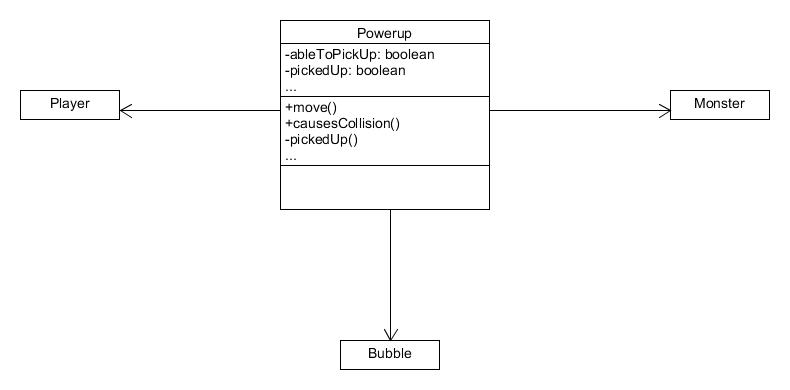
\includegraphics[width=100mm]{uml_powerups.jpg}\\[1cm]
The addition of a powerup is achieved by making a new class. This class is the instance of a powerup, as seen in the game. That is why it extends SpriteBase. 
\\\\
When a powerup is picked up, it triggers an effect. This effects for example Player, by increasing its speed. The relations in the UML above represent these effects.


\subsection{Multiple Lives: Responsibility Driven Design}
\subsection{Multiple Lives: UML}
\subsection{A Score: Responsibility Driven Design}
\subsection{A Score: UML}

\chapter{Design Patterns}
\section{Question 1}

'' Choose two design patterns among those that we saw in class.4 For each chosen design pattern, you must
have a corresponding implementation in your code. If not, refactor your code to include it. Then, per each
chosen design pattern, complete the following points:\\
1. Write a natural language description of why and how the pattern is implemented in your code (5 pts).''

\section{Question 2}

''2. Make a class diagram of how the pattern is structured statically in your code (5 pts).''

\section{Question 3}

\subsection{Sequence Diagram for Strategy}
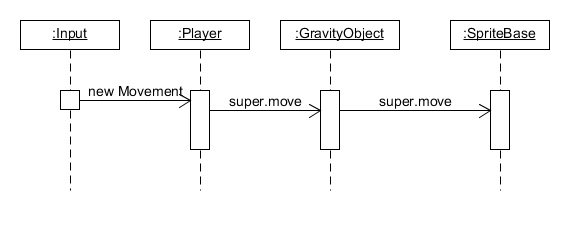
\includegraphics[width=\textwidth]{sequenceDiagramStrategy}

\subsection{Sequence Diagram for Observer}
The observer design pattern, the player has a new movement and he notifies his observers that some change is made.
\begin{figure}[h]
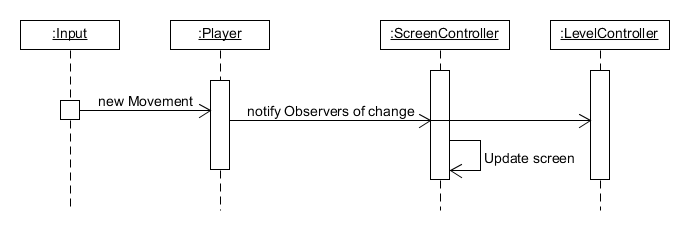
\includegraphics[width=\textwidth]{sequenceDiagramObserver}
\end{figure}

\chapter{Software Engineering Economics}
\section{Question 1}

''Read the paper “How to Build a Good Practice Software Project Portfolio?” available on Blackboard in
the ‘Readings and More’ folder within the ‘Content’ section and answer the following questions:
1. Explain how good and bad practice are recognized (4 pts).''
\section{Question 2}

``Explain why Visual Basic being in the good practice group is a not so interesting finding of the study
(3 pts).'' \\

As described on page 70 of the paper, only 6 projects with the Project Factor ``PPL Visual Basic'' were analysed. Of those 6 projects, 5 scored as a Good Practice and one scored as Cost over Time. Therefore the Project Factor ``PPL Visual Basic'' was selected as one of the factors which relate to Good Practice. As you can see however, the number of samples in this group is too small to conclude that Visual Basics always is a success factor. A good improvement would be to set a minimum sample size $n$ in order to be selected as a success or failure factor.  
\section{Question 3}

\begin{enumerate}
	\item \textbf{Test Driven Development}: This would probably be a good practice. Although Test Driven Development might take more time and could therefore maybe end up in the `Cost over Time'-quarter, it would probably end up as a Good Practice. This is because the developed software will be more maintainable and will be easier to verify for bugs. Because of this, the quality of the software will improve which will mean relatively fewer costs than, for example, when bugs have to be removed at the end. Test Driven Development also means investing a little more time in testing while developing software. This could result in a relatively longer duration, but we are convinced that this little investment of time will result in lower overall duration of the project, since bugs will be found easier and therefore will help prevent more bugs. 
	\item \textbf{Including Design Patterns}: This would probably be good practice mainly due to the same reasons as Test Driven Development. Initially working with Design Patterns might take a bit more time and will require a team with more skills (so more expensive employees). However in the end it will results in easily extendable and more maintainable software which will result in a positive practice. 
	\item \textbf{Visual Development Process}: With this we mean that during the development process, intensive use is made of visualisation (such as UML's) to keep track of for example software structure or model relations. We believe that this will result in a global understanding of the desired structure of the application which will result in lower cost and duration. It is easier to discuss problems, improve software or add new features, once it is understood how the application will be / is constructed. Visualisation is a very good way of doing all of this. 
\end{enumerate}
\section{Question 4}

''4. Describe in detail 3 bad practice factors and why they belong to the bad practice group (4 pts).''
%Your text files go here
\nocite{*}
\bibliographystyle{newapa}
\end{document}